\runningheader{SAT Mathematics}{Drill Set 3}{Page \thepage\ of \numpages}

\begingradingrange{sat-drill-03}
\subsection*{SAT Drill 3}

\question[1]
What is the median of the seven data values shown?
\[
  2,2,2,3,4,4,11
\]
\begin{choices}
  \choice 2
  \CorrectChoice 3
  \choice 4
  \choice 9
\end{choices}

\question[1]
The box plots summarize the masses, in kilograms, of two groups of gazelles.
\phantom{\space}\\

\begin{center}
  
\includegraphics[width=0.90\linewidth]{images/2025_06_15_04f7426dc644de311e92g-02}
\end{center}
Based on the box plots, which of the following statements must be true?
\begin{choices}
  \choice The mean mass of group 1 is greater than the mean mass of group 2.
  \choice The mean mass of group 1 is less than the mean mass of group 2.
  \CorrectChoice The median mass of group 1 is greater than the median mass of group 2.
  \choice The median mass of group 1 is less than the median mass of group 2.
\end{choices}


\newpage


\question[1]
The table below shows the distribution of ages of the 20 students enrolled in a college class. Which of the following gives the correct order of the mean, median, and mode of the ages?
\vspace{0.5em}
\begin{center}
  \renewcommand{\arraystretch}{1.3}
  \setlength{\tabcolsep}{0.5em}
  {\textbf{Ages of 20 Students Enrolled in a College Class}\par}
  \vspace{0.35em}
  \begin{tabular}{|c|c|}
    \hline
    \rowcolor[HTML]{E0E0E0}
    \textbf{Age} & \textbf{Frequency} \\
    \hline
    18 & 6 \\
    \hline 
    19 & 5 \\
    \hline
    20 & 4 \\
    \hline
    21 & 2 \\
    \hline
    22 & 1 \\
    \hline
    23 & 1 \\
    \hline
    30 & 1 \\
    \hline
  \end{tabular}
\end{center}
\begin{choices}
  \CorrectChoice mode $<$ median $<$ mean
  \choice mode $<$ mean $<$ median
  \choice median $<$ mode $<$ mean
  \choice mean $<$ mode $<$ median
\end{choices}



\question[1]
Data set $A$ and data set $B$ each contain 5 numbers.
\[
  \text{Data set A: }72,73,73,76,76
\]
\[
  \text{Data set B: }61, 64, 74, 85, x
\]
If the mean of data set $A$ is equal to the mean of data set $B$, what is the value of $x$?
\begin{choices}
  \choice 77
  \choice 85
  \CorrectChoice 86
  \choice 95
\end{choices}


\newpage


\question[1]
Which frequency table correctly represents the data listed?
\[
  4,4,4,4,8,8,8,13,13
\]
\vspace{0.5em}
\begin{choices}
  \CorrectChoice \parbox[t][7\baselineskip][t]{0.38\linewidth}{\centering
    \begin{tabular}{|c|c|}
      \hline
      Number & Frequency \\
      \hline
      4 & 4 \\
      \hline
      8 & 3 \\
      \hline
      13 & 2 \\
      \hline
    \end{tabular}}
  \choice \parbox[t][7\baselineskip][t]{0.38\linewidth}{\centering
    \begin{tabular}{|c|c|}
      \hline
      Number & Frequency \\
      \hline
      4 & 4 \\
      \hline
      3 & 8 \\
      \hline
      2 & 13 \\
      \hline
    \end{tabular}}
  \choice \parbox[t][7\baselineskip][t]{0.38\linewidth}{\centering
    \begin{tabular}{|c|c|}
      \hline
      Number & Frequency \\
      \hline
      4 & 16 \\
      \hline
      8 & 24 \\
      \hline
      13 & 26 \\
      \hline
    \end{tabular}}
  \choice \parbox[t][7\baselineskip][t]{0.38\linewidth}{\centering
    \begin{tabular}{|c|c|}
      \hline
      Number & Frequency \\
      \hline
      16 & 4 \\
      \hline
      24 & 8 \\
      \hline
      26 & 13 \\
      \hline
    \end{tabular}}
\end{choices}




\newpage



\question[1]
The frequency table summarizes the 57 data values in a data set. What is the maximum data value in the data set?
\vspace{0.5em}
\begin{center}
  \renewcommand{\arraystretch}{1.3}
  \setlength{\tabcolsep}{0.5em}
  {\textbf{Frequency Table}\par}
  \vspace{0.35em}
  \begin{tabular}{|c|c|}
    \hline
    \rowcolor[HTML]{E0E0E0}
    \textbf{Data value} & \textbf{Frequency} \\
    \hline
    6 & 3 \\
    \hline
    7 & 3 \\
    \hline
    8 & 8 \\
    \hline
    9 & 8 \\
    \hline
    10 & 9 \\
    \hline
    11 & 11 \\
    \hline
    12 & 9 \\
    \hline
    13 & 0 \\
    \hline
    14 & 6 \\
    \hline
  \end{tabular}
\end{center}
\begin{solutionorbox}
$14$ (the greatest value that occurs in the data set; $13$ has frequency $0$.)
\end{solutionorbox}


\question[1]
For a school fund-raiser, 10 students sold a total of 90 boxes of cookies. Which of the following can be calculated from this information?
\begin{choices}
  \CorrectChoice The average number of boxes sold per student
  \choice The median number of boxes sold per student
  \choice The greatest number of boxes sold by one student
  \choice The least number of boxes sold by one student
\end{choices}


\newpage


\question[1]
The results of two independent surveys are shown in the table below.
\vspace{0.5em}
\begin{center}
  \renewcommand{\arraystretch}{1.3}
  \setlength{\tabcolsep}{0.5em}
  {\textbf{Men's Height Survey Results}\par}
  \vspace{0.35em}
  \begin{tabular}{|c|c|c|c|}
    \hline
    \rowcolor[HTML]{E0E0E0}
    \textbf{Group} &
    \makecell{\textbf{Sample}\\\textbf{Size}} &
    \makecell{\textbf{Mean}\\\textbf{(cm)}} &
    \makecell{\textbf{Std.\ Dev.}\\\textbf{(cm)}} \\
    \hline
    A & 2,500 & 186 & 12.5 \\
    B & 2,500 & 186 & 19.1 \\
    \hline
  \end{tabular}
\end{center}
Which statement is true based on the table?
\begin{choices}
  \choice The Group A data set was identical to the Group B data set.
  \choice Group B contained the tallest participant.
  \CorrectChoice The heights of the men in Group B had a larger spread than the heights of the men in Group A.
  \choice The median height of Group B is larger than the median height of Group A.
\end{choices}

\question[1]
The mean and the median of the five numbers above are equal.
\[
  15,14,18,17, x
\]
Which of the following is NOT a possible value of $x$?
\begin{choices}
  \CorrectChoice 6
  \choice 11
  \choice 16
  \choice 21
\end{choices}



\question[1]
Each year, the value of an investment increases by $0.49\%$ of its value the previous year. Which of the following functions best models how the value of the investment changes over time?
\begin{choices}
  \choice Decreasing exponential
  \choice Decreasing linear
  \CorrectChoice Increasing exponential
  \choice Increasing linear
\end{choices}



\newpage




\question[1]
Data set A consists of 10 positive integers less than 60. The list shown gives 9 of the integers from data set A.
\[
  43,45,44,43,38,39,40,46,40
\]
The mean of these 9 integers is 42. If the mean of data set A is an integer that is greater than 42, what is the value of the largest integer from data set A?
\begin{solutionorbox}[1.25in]
  $52$
\end{solutionorbox}




\question[1]
Distance and Density of Planetoids in the Inner Solar System
\phantom{\space}\\

\begin{center}
  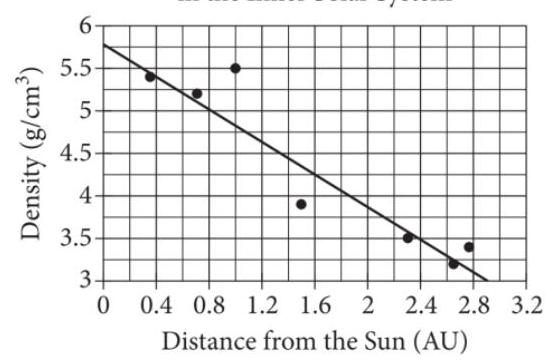
\includegraphics[width=0.90\linewidth]{images/2025_06_15_c6d1fe032100fbb48447g-01}
\end{center}
The scatterplot above shows the densities of 7 planetoids, in grams per cubic centimeter, with respect to their average distances from the Sun in astronomical units (AU). The line of best fit is also shown. An astronomer has discovered a new planetoid about 1.2 AU from the Sun. According to the line of best fit, which of the following best approximates the density of the planetoid, in grams per cubic centimeter?
\begin{choices}
  \choice 3.6
  \choice 4.1
  \CorrectChoice 4.6
  \choice 5.5
\end{choices}


\newpage


\question[1]
The scatterplot shows the relationship between $x$ and $y$. A line of best fit is also shown.
\phantom{\space}\\

\begin{center}
  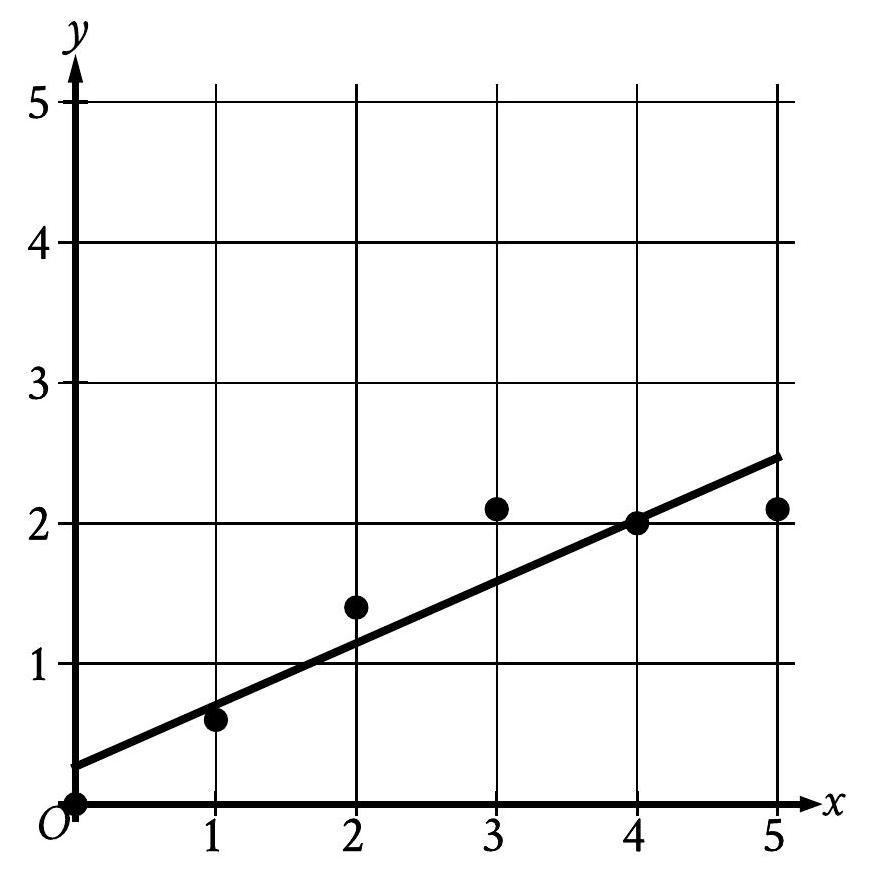
\includegraphics[width=0.90\linewidth]{images/2025_06_15_c6d1fe032100fbb48447g-03}
\end{center}
Which of the following is closest to the slope of the line of best fit shown?
\begin{choices}
  \choice $-2.27$
  \CorrectChoice $-0.44$
  \choice $0.44$
  \choice $2.27$
\end{choices}


\newpage




\question[1]
\phantom{\space}\\
\begin{center}
  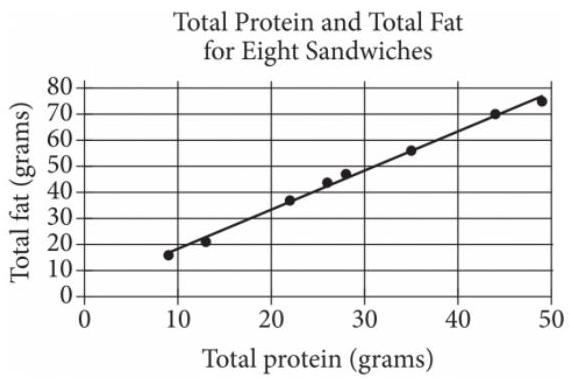
\includegraphics[width=0.90\linewidth]{images/2025_06_15_c6d1fe032100fbb48447g-04}
\end{center}
The scatterplot above shows the numbers of grams of both total protein and total fat for eight sandwiches on a restaurant menu. The line of best fit for the data is also shown. According to the line of best fit, which of the following is closest to the predicted increase in total fat, in grams, for every increase of 1 gram in total protein?
\begin{choices}
  \choice 2.5
  \choice 2.0
  \CorrectChoice 1.5
  \choice 1.0
\end{choices}





\newpage




\question[1]
The scatterplot shows the relationship between two variables, $x$ and $y$.
\phantom{\space}\\

\begin{center}
  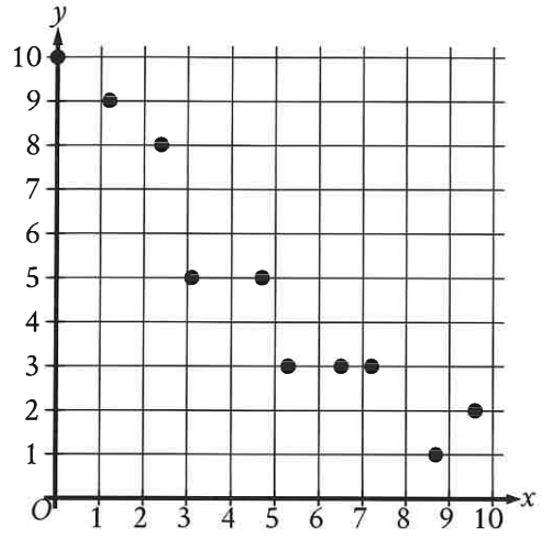
\includegraphics[width=0.90\linewidth]{images/cus12}
\end{center}
Which of the following equations is the most appropriate linear model for the data shown?
\begin{choices}
  \choice $y=0.9+9.4 x$
  \choice $y=0.9-9.4 x$
  \choice $y=9.4+0.9 x$
  \CorrectChoice $y=9.4-0.9 x$
\end{choices}


\question[1]
For $x>0$, the function $f$ is defined as follows:
\[
  f(x) \text{ equals } 201\% \text{ of } x
\]
Which of the following could describe this function?
\begin{choices}
  \choice Decreasing exponential
  \choice Decreasing linear
  \choice Increasing exponential
  \CorrectChoice Increasing linear
\end{choices}




\newpage




\question[1]
\phantom{\space}\\
\begin{center}
  \renewcommand{\arraystretch}{1.3}
  \setlength{\tabcolsep}{0.5em} 
  {\textbf{Investment Comparison}\par}
  \vspace{0.35em}
  \begin{tabular}{|c|c|c|}
    \hline
    \rowcolor[HTML]{E0E0E0}
    \mbox{} &
    \begin{tabular}{@{}c@{}}\textbf{Amount}\\\textbf{invested}\end{tabular} &
    \begin{tabular}{@{}c@{}}\textbf{Balance}\\\textbf{increase}\end{tabular} \\
    \hline
    Account A & $\$ 500$ & $6\%$ annual interest \\
    \hline
    Account B & $\$ 1,000$ & $\$ 25$ per year \\
    \hline
  \end{tabular}
\end{center}
Two investments were made as shown in the table above. The interest in Account A is compounded once per year. Which of the following is true about the investments?
\begin{choices}
  \CorrectChoice Account A always earns more money per year than Account B.
  \choice Account A always earns less money per year than Account B.
  \choice Account A earns more money per year than Account B at first but eventually earns less money per year.
  \choice Account A earns less money per year than Account B at first but eventually earns more money per year.
\end{choices}


\newpage


\question[1]
The scatterplot shows the relationship between two variables, $x$ and $y$. A line of best fit for the data is also shown.
\phantom{\space}\\

\begin{center}
  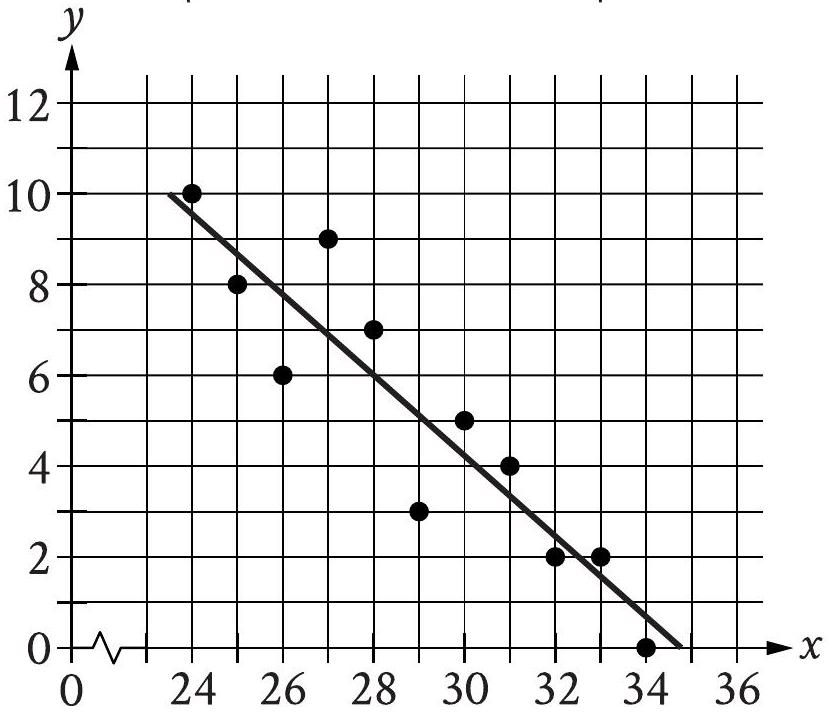
\includegraphics[width=0.90\linewidth]{images/2025_06_15_c6d1fe032100fbb48447g-08}
\end{center}
At $x=32$, which of the following is closest to the $y$-value predicted by the line of best fit?
\begin{choices}
  \choice 0.4
  \choice 1.5
  \CorrectChoice 2.4
  \choice 3.3
\end{choices}


\newpage


\question[1]
\phantom{\space}\\
\begin{center}
  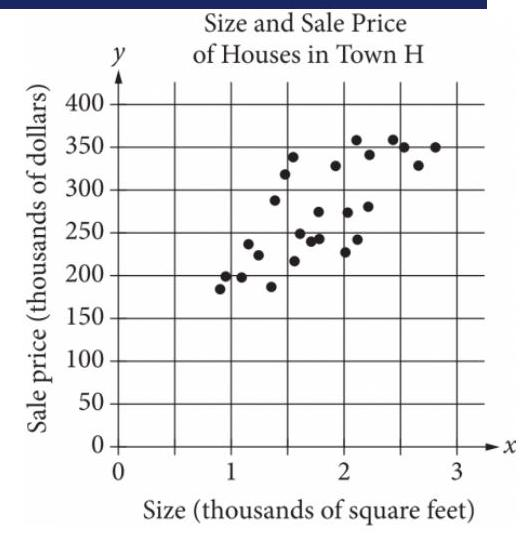
\includegraphics[width=0.90\linewidth]{images/2025_06_15_c6d1fe032100fbb48447g-09}
\end{center}
The scatterplot above shows the size $x$ and the sale price $y$ of 25 houses for sale in Town H. Which of the following could be an equation for a line of best fit for the data?
\begin{choices}
  \choice $y=200 x+100$
  \CorrectChoice $y=100 x+100$
  \choice $y=50 x+100$
  \choice $y=100 x$
\end{choices}




\newpage



\question[1]
\phantom{\space}\\

\begin{center}
  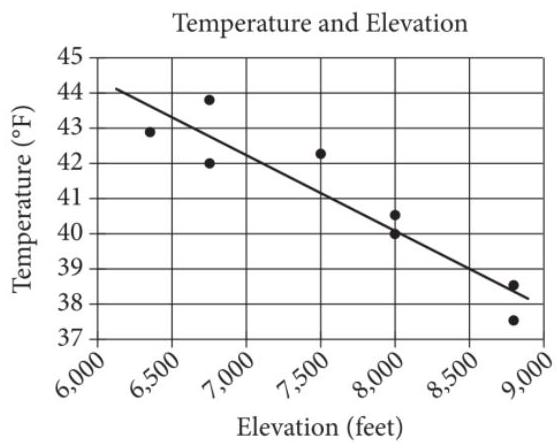
\includegraphics[width=0.90\linewidth]{images/2025_06_15_c6d1fe032100fbb48447g-10}
\end{center}
The scatterplot above shows the high temperature on a certain day and the elevation of 8 different locations in the Lake Tahoe Basin. A line of best fit for the data is also shown. Which of the following statements best describes the association between the elevation and the temperature of locations in the Lake Tahoe Basin?
\begin{choices}
  \choice As the elevation increases, the temperature tends to increase.
  \CorrectChoice As the elevation increases, the temperature tends to decrease.
  \choice As the elevation decreases, the temperature tends to decrease.
  \choice There is no association between the elevation and the temperature.
\end{choices}

\question[1]
A printer produces posters at a constant rate of 42 posters per minute. At what rate, in posters per hour, does the printer produce the posters?
\begin{solutionorbox}[1.25in]
  $2{,}520$
\end{solutionorbox}




\newpage



\question[1]
The International Space Station orbits Earth at an average speed of 4.76 miles per second. What is the space station's average speed in miles per hour?
\begin{choices}
  \choice 285.6
  \choice 571.2
  \choice 856.8
  \CorrectChoice $17136.0$
\end{choices}



\question[1]
For a person $m$ miles from a flash of lightning, the length of the time interval from the moment the person sees the lightning to the moment the person hears the thunder is $k$ seconds. The ratio of $m$ to $k$ can be estimated to be 1 to 5. According to this estimate, the person is how many miles from a flash of lightning if the time interval is 25 seconds?
\begin{choices}
  \choice 10
  \choice 9
  \choice 6
  \CorrectChoice 5
\end{choices}

\question[1]
The population density of Iceland, in people per square kilometer of land area, increased from 2.5 in 1990 to 3.3 in 2014. During this time period, the land area of Iceland was 100,250 square kilometers. By how many people did Iceland's population increase from 1990 to 2014?
\begin{choices}
  \choice 330,825
  \choice 132,330
  \choice 125,312
  \CorrectChoice 80,200
\end{choices}


\newpage



\question[1]
A customer spent $\$ 27$ to purchase oranges at $\$ 3$ per pound. How many pounds of oranges did the customer purchase?
\begin{solutionorbox}[1.25in]
  $9$
\end{solutionorbox}

\question[1]
A group of monarch butterflies migrated from Chicago, Illinois, to Michoacán, Mexico, flying a total of 2,100 miles. It took a single butterfly in the group 120 days to travel this route one way. On average, how many miles did the butterfly travel per day?
\begin{choices}
  \choice 0.057
  \choice 0.729
  \CorrectChoice 17.5
  \choice 24
\end{choices}

\question[1]
If $\frac{x}{y}=4$ and $\frac{24 x}{n y}=4$, what is the value of $n$?
\begin{solutionorbox}[1.25in]
  $24$
\end{solutionorbox}

\question[1]
In a box of pens, the ratio of black pens to red pens is 8 to 1. There are 40 black pens in the box. How many red pens are in the box?
\begin{choices}
  \CorrectChoice 5
  \choice 8
  \choice 40
  \choice 320
\end{choices}

\question[1]
Pure beeswax has a density of 0.555 ounce per cubic inch. An online company sells pure beeswax at a price of $\$ 8.00$ per ounce. What is the selling price, in dollars per cubic inch, for pure beeswax purchased from this company?
\begin{solutionorbox}[1.25in]
  $\$ 4.44$
\end{solutionorbox}




\question[1]
The population density of Worthington is 290 people per square mile. Worthington has a population of 92,800 people. What is the area, in square miles, of Worthington?
\begin{choices}
  \choice 102,400
  \choice 93,090
  \CorrectChoice 320
  \choice 32
\end{choices}

\question[1]
Jennifer bought a box of Crunchy Grain cereal. The nutrition facts on the box state that a serving size of the cereal is $\frac{3}{4}$ cup and provides 210 calories, 50 of which are calories from fat. In addition, each serving of the cereal provides 180 milligrams of potassium, which is $5\%$ of the daily allowance for adults. If $p$ percent of an adult's daily allowance of potassium is provided by $x$ servings of Crunchy Grain cereal per day, which of the following expresses $p$ in terms of $x$?
\begin{choices}
  \choice $p=0.5 x$
  \CorrectChoice $p=5 x$
  \choice $p=(0.05)^{x}$
  \choice $p=(1.05)^{x}$
\end{choices}



\newpage


\question[1]
A school district is forming a committee to discuss plans for the construction of a new high school. Of those invited to join the committee, 15\% are parents of students, 45\% are teachers from the current high school, 25\% are school and district administrators, and the remaining 6 individuals are students. How many more teachers were invited to join the committee than school and district administrators?
\begin{solutionorbox}[1.25in]
  $8$
\end{solutionorbox}





\question[1]
A table of the US minimum wage for 6 different years is shown below.
\vspace{0.5em}
\begin{center}
  \renewcommand{\arraystretch}{1.3}
  \setlength{\tabcolsep}{0.5em}
  {\textbf{US Minimum Wage by Year}\par}
  \vspace{0.35em}
  \begin{tabular}{|c|c|}
    \hline
    \rowcolor[HTML]{E0E0E0} 
    \textbf{Year} &
    \begin{tabular}{@{}c@{}}\textbf{US Minimum Wage}\\\textbf{(dollars per hour)}\end{tabular} \\
    \hline
    1960 & \$1.00 \\
    \hline
    1970 & \$1.60 \\
    \hline
    1980 & \$3.10 \\
    \hline
    1990 & \$3.80 \\
    \hline
    2000 & \$5.15 \\
    \hline
    2010 & \$7.25 \\
    \hline
  \end{tabular}
\end{center}
What was the percent increase of the minimum wage from 1960 to 1970?
\begin{choices}
  \choice $30\%$
  \CorrectChoice $60\%$
  \choice $62.5\%$
  \choice $120\%$
\end{choices}



\newpage


\question[1]
The manager of an online news service received the report below on the number of subscriptions sold by the service. The manager estimated that the percent increase from 2012 to 2013 would be double the percent increase from 2013 to 2014. How many subscriptions did the manager expect would be sold in 2014?
\vspace{0.5em}
\begin{center}
  \renewcommand{\arraystretch}{1.3}
  \setlength{\tabcolsep}{0.5em}
  {\textbf{Subscription Sales}\par}
  \vspace{0.35em}
  \begin{tabular}{|c|c|}
    \hline
    \rowcolor[HTML]{E0E0E0}
    \textbf{Year} & \textbf{Subscriptions sold} \\
    \hline
    2012 & 5,600 \\
    \hline
    2013 & 5,880 \\
    \hline
  \end{tabular}
\end{center}
\begin{choices}
  \choice 6,020
  \CorrectChoice 6,027
  \choice 6,440
  \choice 6,468
\end{choices}

\question[1]
The line graph shows the total amount of snow, in inches, recorded each year in Washington, DC, from 2003 to 2015. If $p\%$ is the percent decrease in the annual snowfall from 2003 to 2007, what is the value of $p$?
\begin{center}
  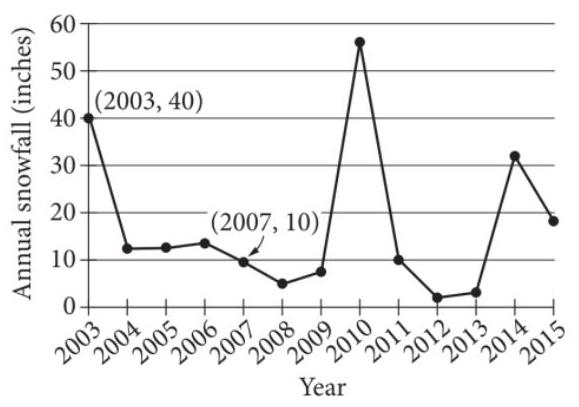
\includegraphics[width=0.90\linewidth]{images/2025_06_15_685e39be57606e31d5a9g-05}
\end{center}
\begin{solutionorbox}[1.25in]
  $40$
\end{solutionorbox}



\newpage



\question[1]
What percentage of 300 is 75?
\begin{choices}
  \CorrectChoice $25\%$
  \choice $50\%$
  \choice $75\%$
  \choice $225\%$
\end{choices}

\question[1]
The cost of a certain shirt is \$20 before a 5\% sales tax is added. What is the total cost, including sales tax, to purchase the shirt?
\begin{choices}
  \choice $\$ 20.05$
  \choice $\$ 20.50$
  \CorrectChoice $\$ 21.00$
  \choice $\$ 25.00$
\end{choices}

\question[1]
For the finale of a TV show, viewers could use either social media or a text message to vote for their favorite of two contestants. The contestant receiving more than $50\%$ of the vote won. An estimated $10\%$ of the viewers voted, and $30\%$ of the votes were cast on social media. Contestant 2 earned $70\%$ of the votes cast using social media and $40\%$ of the votes cast using a text message. Based on this information, which of the following is an accurate conclusion?
\begin{choices}
  \choice If all viewers had voted, Contestant 2 would have won.
  \choice Viewers voting by social media were likely to be younger than viewers voting by text message.
  \choice If all viewers who voted had voted by social media instead of by text message, Contestant 2 would have won.
  \CorrectChoice Viewers voting by social media were more likely to prefer Contestant 2 than were viewers voting by text message.
\end{choices}

\question[1]
During the first month of sales, a company sold 1,300,000 units of a certain type of smartphone. During the same month, $15\%$ of the units sold were returned. If sales and the return rate remain the same for each of the next 5 months, about how many units of this smartphone will be returned to the company during this 6-month period?
\begin{choices}
  \choice 195,000
  \choice 975,000
  \CorrectChoice $1{,}170{,}000$
  \choice $6{,}630{,}000$
\end{choices}

\question[1]
Last year, 200 students enrolled in an interior design program. This year, the number of students enrolled is $147\%$ of last year's number. How many students are enrolled in the interior design program this year?
\begin{choices}
  \choice 247
  \CorrectChoice 294
  \choice 347
  \choice 394
\end{choices}



\question[1]
There are 55 students in Spanish club. A sample of the Spanish club students was selected at random and asked whether they intend to enroll in a new study program. Of those surveyed, $20\%$ responded that they intend to enroll in the study program. Based on this survey, which of the following is the best estimate of the total number of Spanish club students who intend to enroll in the study program?
\begin{choices}
  \CorrectChoice 11
  \choice 20
  \choice 44
  \choice 55
\end{choices}






\newpage

\question[1]
In a study of cell phone use, 799 randomly selected US teens were asked how often they talked on a cell phone and about their texting behavior. The data are summarized in the table above. Based on the data from the study, an estimate of the percent of US teens who are heavy texters is $30\%$ and the associated margin of error is $3\%$. Which of the following is a correct statement based on the given margin of error?
\vspace{0.5em}
\begin{center}
  \renewcommand{\arraystretch}{1.3}
  \setlength{\tabcolsep}{0.5em}
  {\textbf{Cell Phone Use Study}\par}
  \vspace{0.35em}
  \begin{adjustbox}{max width=\linewidth,clip=false,margin=1pt}
  \begin{tabular}{|c|c|c|c|}
    \hline
    \cellcolor[HTML]{E0E0E0}\begin{tabular}{@{}c@{}}\textbf{Texting}\\\textbf{behavior}\end{tabular} &
    \cellcolor[HTML]{E0E0E0}\begin{tabular}{@{}c@{}}\textbf{Talks on}\\\textbf{cell phone}\\\textbf{daily}\end{tabular} &
    \cellcolor[HTML]{E0E0E0}\begin{tabular}{@{}c@{}}\textbf{Does not}\\\textbf{talk on}\\\textbf{cell phone}\\\textbf{daily}\end{tabular} &
    \cellcolor[HTML]{E0E0E0}\begin{tabular}{@{}c@{}}\textbf{Total}\end{tabular} \\
    \hline
    Light & 110 & 146 & 256 \\
    \hline
    Medium & 139 & 164 & 303 \\
    \hline
    Heavy & 166 & 74 & 240 \\
    \hline
    Total & 415 & 384 & 799 \\
    \hline
  \end{tabular}
  \end{adjustbox}
\end{center}
\begin{choices}
  \choice Approximately $3\%$ of the teens in the study who are classified as heavy texters are not really heavy texters.
  \choice It is not possible that the percent of all US teens who are heavy texters is less than $27\%$.
  \choice The percent of all US teens who are heavy texters is $33\%$.
  \CorrectChoice It is doubtful that the percent of all US teens who are heavy texters is $35\%$.
\end{choices}



\newpage


\question[1]
A researcher interviewed 411 randomly selected US residents and asked about their views on the use of nuclear energy. The table above summarizes the responses of the interviewees. If the population of the United States was 300 million when the survey was given, based on the sample data for the 411 US residents, what is the best estimate, in millions, of the difference between the number of US residents who somewhat favor or strongly favor the use of nuclear energy and the number of those who somewhat oppose or strongly oppose it? (Round your answer to the nearest whole number.)
\vspace{0.5em}
\begin{center}
  \renewcommand{\arraystretch}{1.3} 
  \setlength{\tabcolsep}{0.5em}
  {\textbf{Views on Nuclear Energy}\par}
  \vspace{0.35em}
  \begin{tabular}{|l|c|}
    \hline
    \rowcolor[HTML]{E0E0E0}
    \textbf{Response} & \textbf{Frequency} \\
    \hline
    Strongly favor    & 56  \\
    Somewhat favor    & 214 \\
    Somewhat oppose   & 104 \\
    Strongly oppose   & 37  \\
    \hline
  \end{tabular}
\end{center}
\begin{solutionorbox}[1.25in]
  $94$
\end{solutionorbox}

\newpage

\question[1]
The same 20 contestants, on each of 3 days, answered 5 questions in order to win a prize. Each contestant received 1 point for each correct answer. The number of contestants receiving a given score on each day is shown in the table above. No contestant received the same score on two different days. If a contestant is selected at random, what is the probability that the selected contestant received a score of 5 on Day 2 or Day 3, given that the contestant received a score of 5 on one of the three days?
\vspace{0.5em}
\begin{center}
  \renewcommand{\arraystretch}{1.3}
  \setlength{\tabcolsep}{0.5em}
  {\textbf{Number of Contestants by Score and Day}\par}
  {\small(Each score is out of 5.)\par}
  \vspace{0.35em}
  \begin{adjustbox}{max width=\linewidth,clip=false,margin=1pt}
  \begin{tabular}{|c|c|c|c|c|c|c|c|}
    \hline
    \cellcolor[HTML]{E0E0E0}\mbox{} &
    \cellcolor[HTML]{E0E0E0}\textbf{5} &
    \cellcolor[HTML]{E0E0E0}\textbf{4} &
    \cellcolor[HTML]{E0E0E0}\textbf{3} &
    \cellcolor[HTML]{E0E0E0}\textbf{2} &
    \cellcolor[HTML]{E0E0E0}\textbf{1} &
    \cellcolor[HTML]{E0E0E0}\textbf{0} &
    \cellcolor[HTML]{E0E0E0}\textbf{Total} \\
    \hline
    Day 1 & 2 & 3 & 4 & 6 & 2 & 3 & 20 \\
    \hline
    Day 2 & 2 & 3 & 5 & 5 & 4 & 1 & 20 \\
    \hline
    Day 3 & 3 & 3 & 4 & 5 & 3 & 2 & 20 \\
    \hline
    Total & 7 & 9 & 13 & 16 & 9 & 6 & 60 \\
    \hline
  \end{tabular}
  \end{adjustbox}
\end{center}
\begin{solutionorbox}[1.25in]
  $\dfrac{5}{7}$
\end{solutionorbox}

\question[1]
Each face of a fair 14-sided die is labeled with a number from 1 through 14, with a different number appearing on each face. If the die is rolled one time, what is the probability of rolling a 2?
\begin{choices}
  \CorrectChoice $\dfrac{1}{14}$
  \choice $\dfrac{2}{14}$
  \choice $\dfrac{12}{14}$
  \choice $\dfrac{13}{14}$
\end{choices}

\newpage

\question[1]
The table below shows information about 14 cars listed for sale on an auto dealership's website. If one of the cars listed for sale is selected at random, what is the probability that the car selected will be a hybrid car priced at no more than $\$ 25,000$?
\vspace{0.5em}
\begin{center}
  \renewcommand{\arraystretch}{1.3}
  \setlength{\tabcolsep}{0.5em}
  {\textbf{Prices of 14 Different Cars}\par}
  \vspace{0.35em}
  \begin{adjustbox}{max width=\linewidth,clip=false,margin=1pt}
  \begin{tabular}{|c|c|c|c|}
    \hline
    \cellcolor[HTML]{E0E0E0}\begin{tabular}{@{}c@{}}\textbf{Type}\\\textbf{of}\\\textbf{car}\end{tabular} &
    \cellcolor[HTML]{E0E0E0}\begin{tabular}{@{}c@{}}\textbf{Priced}\\\textbf{at no more}\\\textbf{than}\\\textbf{\$25,000}\end{tabular} &
    \cellcolor[HTML]{E0E0E0}\begin{tabular}{@{}c@{}}\textbf{Priced}\\\textbf{greater}\\\textbf{than \$25,000}\end{tabular} &
    \cellcolor[HTML]{E0E0E0}\textbf{Total} \\
    \hline
    Nonhybrid & 5 & 3 & 8 \\
    \hline
    Hybrid & 2 & 4 & 6 \\
    \hline
    Total & 7 & 7 & 14 \\
    \hline
  \end{tabular}
  \end{adjustbox}
\end{center}
\begin{choices}
  \CorrectChoice $\dfrac{1}{7}$
  \choice $\dfrac{2}{7}$
  \choice $\dfrac{1}{3}$
  \choice $\dfrac{4}{7}$
\end{choices}

\question[1]
The table below shows the number of different colors of marbles in a bag. If a marble is chosen at random from the bag, what is the probability that the marble will be blue?
\vspace{0.5em}
\begin{center}
  \renewcommand{\arraystretch}{1.3}
  \setlength{\tabcolsep}{0.5em}
  {\textbf{Colors of Marbles in a Bag}\par}
  \vspace{0.35em}
  \begin{tabular}{|c|c|}
    \hline
    \rowcolor[HTML]{E0E0E0}
    \textbf{Color} & \textbf{Number} \\
    \hline
    Red & 8 \\
    \hline
    Blue & 10 \\
    \hline
    Green & 22 \\
    \hline
    Total & 40 \\
    \hline
  \end{tabular}
\end{center}
\begin{choices}
  \choice $\dfrac{30}{40}$
  \choice $\dfrac{22}{40}$
  \choice $\dfrac{18}{40}$
  \CorrectChoice $\dfrac{10}{40}$
\end{choices}

\newpage

\question[1]
On Tuesday, a local gas station had 135 customers. The table above summarizes whether or not the customers on Tuesday purchased gasoline, a beverage, both, or neither. Based on the data in the table, what is the probability that a gas station customer selected at random on that day did not purchase gasoline?
\vspace{0.5em}
\begin{center}
  \renewcommand{\arraystretch}{1.3}
  \setlength{\tabcolsep}{0.5em}
  {\textbf{Customer Purchases at a Gas Station}\par}
  \vspace{0.35em}
  \begin{adjustbox}{max width=\linewidth,clip=false,margin=1pt}
  \begin{tabular}{|c|c|c|c|}
    \hline
    \cellcolor[HTML]{E0E0E0}\mbox{} &
    \cellcolor[HTML]{E0E0E0}\begin{tabular}{@{}c@{}}\textbf{Beverage}\\\textbf{purchased}\end{tabular} &
    \cellcolor[HTML]{E0E0E0}\begin{tabular}{@{}c@{}}\textbf{Beverage}\\\textbf{not}\\\textbf{purchased}\end{tabular} &
    \cellcolor[HTML]{E0E0E0}\textbf{Total} \\
    \hline
    \begin{tabular}{@{}c@{}}Gasoline\\purchased\end{tabular} & 60 & 25 & 85 \\
    \hline
    \begin{tabular}{@{}c@{}}Gasoline\\not\\purchased\end{tabular} & 35 & 15 & 50 \\
    \hline
    Total & 90 & 40 & 135 \\
    \hline
  \end{tabular}
  \end{adjustbox}
\end{center}
\begin{choices}
  \choice $\dfrac{15}{50}$
  \choice $\dfrac{15}{40}$
  \choice $\dfrac{35}{50}$
  \CorrectChoice $\dfrac{50}{135}$
\end{choices}

\question[1]
A sample of 40 fourth-grade students was selected at random from a certain school. The 40 students completed a survey about the morning announcements, and 32 thought the announcements were helpful. Which of the following is the largest population to which the results of the survey can be applied?
\begin{choices}
  \choice The 40 students who were surveyed
  \CorrectChoice All fourth-grade students at the school
  \choice All students at the school
  \choice All fourth-grade students in the county in which the school is located
\end{choices}

\question[1]
Residents of a town were surveyed to determine whether they are satisfied with the concession stand at the local park. A random sample of 200 residents was selected. All 200 responded, and $87\%$ said they are satisfied. Based on this information, which of the following statements must be true?
\statementbox{
  \begin{enumerate}[label=(\Roman*)]
    \item Of all the town residents, $87\%$ would say they are satisfied with the concession stand at the local park.
    \item If another random sample of 200 residents were surveyed, $87\%$ would say they are satisfied.
  \end{enumerate}
}
\begin{choices}
  \CorrectChoice Neither
  \choice I only
  \choice II only
  \choice I and II
\end{choices}

\endgradingrange{sat-drill-03}
